%保存为UTF-8编码格式
%用xelatex编译
 
\documentclass[UTF8,a4paper,12pt]{ctexart}
\usepackage[left=2.50cm, right=2.50cm, top=2.50cm, bottom=2.50cm]{geometry} %页边距
\CTEXsetup[format={\Large\bfseries}]{section} %设置章标题字号为Large,居左
%\CTEXsetup[number={\chinese{section}}]{section}
%\CTEXsetup[name={(,)}]{subsection}
%\CTEXsetup[number={\chinese{subsection}}]{subsection}
%\CTEXsetup[name={(,)}]{subsubsection}
%\CTEXsetup[number=\arabic{subsubsection}]{subsubsection}  %以上四行为各级标题样式设置,可根据需要做修改
 
%\linespread{1.5} %设置全文行间距
 
 
%\usepackage[english]{babel}
%\usepackage{float}     %放弃美学排版图表
\usepackage{fontspec}   %修改字体
\usepackage{amsmath, amsfonts, amssymb} % 数学公式相关宏包
\usepackage{color}      % color content
\usepackage{graphicx}   % 导入图片
\usepackage{subfigure}  % 并排子图
\usepackage{url}        % 超链接
\usepackage{bm}         % 加粗部分公式,比如\bm{aaa}aaa
\usepackage{multirow}
\usepackage{booktabs}
\usepackage{epstopdf}
\usepackage{epsfig}
\usepackage{longtable}  %长表格
\usepackage{supertabular}%跨页表格
\usepackage{algorithm}
\usepackage{algorithmic}
\usepackage{changepage}
 
 
 
%%%%%%%%%%%%%%%%%%%%%%%
% -- text font --
% compile using Xelatex
%%%%%%%%%%%%%%%%%%%%%%%
% -- 中文字体 --
%\setCJKmainfont{Microsoft YaHei}  % 微软雅黑
%\setCJKmainfont{YouYuan}  % 幼圆
%\setCJKmainfont{NSimSun}  % 新宋体
%\setCJKmainfont{KaiTi}    % 楷体
\setCJKmainfont[AutoFakeBold=true]{SimSun}   % 宋体
%\setCJKmainfont{SimHei}   % 黑体
 
% -- 英文字体 --
\setmainfont{Times New Roman}
%\setmainfont{DejaVu Sans}
%\setmainfont{Latin Modern Mono}
%\setmainfont{Consolas}
%
%
\renewcommand{\algorithmicrequire}{ \textbf{Input:}}     % use Input in the format of Algorithm
\renewcommand{\algorithmicensure}{ \textbf{Initialize:}} % use Initialize in the format of Algorithm
\renewcommand{\algorithmicreturn}{ \textbf{Output:}}     % use Output in the format of Algorithm
\renewcommand{\abstractname}{\textbf{\large {摘\quad 要}}} %更改摘要二字的样式
\newcommand{\xiaosi}{\fontsize{12pt}{\baselineskip}}     %\xiaosi代替设置12pt字号命令,不加\selectfont,行间距设置无效
\newcommand{\wuhao}{\fontsize{10.5pt}{10.5pt}\selectfont}
 
\usepackage{fancyhdr} %设置全文页眉、页脚的格式
\pagestyle{fancy}
\lhead{}           %页眉左边设为空
\chead{}           %页眉中间
\rhead{}           %页眉右边
%\rhead{\includegraphics[width=1.2cm]{1.eps}}  %页眉右侧放置logo
\lfoot{}          %页脚左边
\cfoot{\thepage}  %页脚中间
\rfoot{}          %页脚右边
 
 
%%%%%%%%%%%%%%%%%%%%%%%
%  设置水印
%%%%%%%%%%%%%%%%%%%%%%%
%\usepackage{draftwatermark}         % 所有页加水印
%\usepackage[firstpage]{draftwatermark} % 只有第一页加水印
% \SetWatermarkText{Water-Mark}           % 设置水印内容
% \SetWatermarkText{\includegraphics{fig/ZJDX-WaterMark.eps}}         % 设置水印logo
% \SetWatermarkLightness{0.9}             % 设置水印透明度 0-1
% \SetWatermarkScale{1}                   % 设置水印大小 0-1
 
\usepackage{hyperref} %bookmarks
\hypersetup{colorlinks, bookmarks, unicode} %unicode
 
 
 
\title{\textbf{\Large{车辆租赁管理系统实验报告}}}
\author{ 林杰泓 22336137\\刘艺凡 22336162}
%\date{\today}
%\date{2021/10/21}
 
 
 
\begin{document}
 
\maketitle
%\tableofcontents
 
% \begin{abstract}
% 本模板可以提供一般性单栏文档的生成,可以根据需要选择是否要目录、摘要,可自行选择日期生成方式,参考文献使用交叉引用条目形式使用,便于编辑和管理。务必注意,latex编译器需要选择xelatex.
% \end{abstract}
 
% \begin{center}
% \large{\textbf{Abstract}}
% \end{center}
 
% \begin{adjustwidth}{1cm}{1cm}
% \hspace{1.5em}Here is the first par. of abstract.Here is the first par. of abstract.
 
% \noindent\hspace{1.5em}Here is the second par. of abstract.Here is the second par. of abstract.
% \end{adjustwidth}
 
%\thispagestyle{empty}       %本页不显示页码
%\newpage                    %分页
%%\tableofcontents\thispagestyle{empty}
%\newpage
%\setcounter{page}{1}        %从下面开始编页,页脚格式为导言部分设置的格式
\newpage 
\tableofcontents
\newpage
\section{实验题目}
设计一个车辆租赁管理系统,包括车辆信息管理、租赁管理、客户管理等功能。车辆信息管理负责车辆
信息的添加、修改和查询;租赁管理负责租赁信息的录入、修改和查询;客户管理负责客户信息的添
加、修改和查询。
\section{需求分析}

功能需求:

\begin{itemize}
    \item 车辆信息管理:包括车辆的添加、修改、查询。每辆车有编号、品牌、型号、车牌号、租金等信息。
    \item 租赁管理:包括租赁记录的管理,租赁客户、租赁车辆等。
    \item 客户管理:管理客户信息,包含客户ID、姓名、联系方式等。
\end{itemize}

非功能需求:

\begin{itemize}
    \item 安全性:对用户的权限进行控制,确保只有管理员可以进行修改操作。
    \item 系统响应时间:保证系统能快速响应用户操作,尤其是查询操作。
    \item 界面友好性:设计直观的用户界面,保证用户能够方便地操作和管理信息。
\end{itemize}

\subsection{系统结构图}

\begin{figure}[htbp]  % figure 环境用于插入图片并进行浮动
    \centering  % 图片居中
    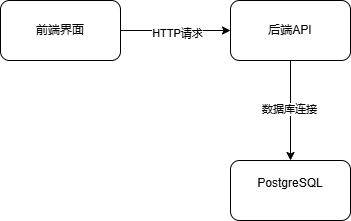
\includegraphics[width=1\textwidth]{pic/sap.png}  % 设置图片宽度为文档宽度的一半
    \caption{系统结构图}  % 图片标题
    \label{fig:sap}  % 图片标签,便于引用
\end{figure}

针对需求分析,我们得到了系统结构图,如图\ref{fig:sap}所示。

\subsection{系统功能模块图}

\begin{figure}[htbp]  % figure 环境用于插入图片并进行浮动
    \centering  % 图片居中
    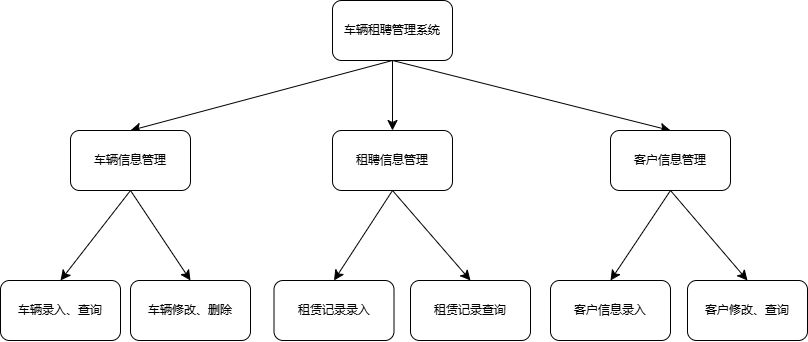
\includegraphics[width=1\textwidth]{pic/system_function_modules.png}  % 设置图片宽度为文档宽度的一半
    \caption{系统功能模块图}  % 图片标题
    \label{fig:sfm}  % 图片标签,便于引用
\end{figure}

针对需求分析,我们得到了系统的功能模块图,如图\ref{fig:sfm}所示。

\subsection{E-R图}

\begin{figure}[htbp]  % figure 环境用于插入图片并进行浮动
    \centering  % 图片居中
    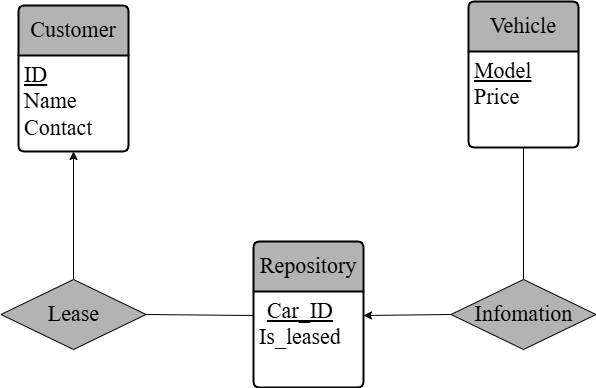
\includegraphics[width=1\textwidth]{pic/er.png}  % 设置图片宽度为文档宽度的一半
    \caption{E-R图}  % 图片标题
    \label{fig:er}  % 图片标签,便于引用
\end{figure}

针对需求分析,画出E-R图表示的概念模型,如图\ref{fig:er}所示。

\subsection{数据库模式}
 
\section{数据库的保护}

\subsection{安全性}

\subsection{完备性}


\end{document}

